%!TEX TS-program = xelatex

% Шаблон документа LaTeX создан в 2018 году
% Алексеем Подчезерцевым
% В качестве исходных использованы шаблоны
% 	Данилом Фёдоровых (danil@fedorovykh.ru) 
%		https://www.writelatex.com/coursera/latex/5.2.2
%	LaTeX-шаблон для русской кандидатской диссертации и её автореферата.
%		https://github.com/AndreyAkinshin/Russian-Phd-LaTeX-Dissertation-Template

\documentclass[a4paper,14pt]{article}


%%% Работа с русским языком
\usepackage[english,russian]{babel}   %% загружает пакет многоязыковой вёрстки
\usepackage{fontspec}      %% подготавливает загрузку шрифтов Open Type, True Type и др.
\defaultfontfeatures{Ligatures={TeX},Renderer=Basic}  %% свойства шрифтов по умолчанию
\setmainfont[Ligatures={TeX,Historic}]{Times New Roman} %% задаёт основной шрифт документа
\setsansfont{Comic Sans MS}                    %% задаёт шрифт без засечек
\setmonofont{Courier New}
\usepackage{indentfirst}
\frenchspacing

\renewcommand{\epsilon}{\ensuremath{\varepsilon}}
\renewcommand{\phi}{\ensuremath{\varphi}}
\renewcommand{\kappa}{\ensuremath{\varkappa}}
\renewcommand{\le}{\ensuremath{\leqslant}}
\renewcommand{\leq}{\ensuremath{\leqslant}}
\renewcommand{\ge}{\ensuremath{\geqslant}}
\renewcommand{\geq}{\ensuremath{\geqslant}}
\renewcommand{\emptyset}{\varnothing}

%%% Дополнительная работа с математикой
\usepackage{amsmath,amsfonts,amssymb,amsthm,mathtools} % AMS
\usepackage{icomma} % "Умная" запятая: $0,2$ --- число, $0, 2$ --- перечисление

%% Номера формул
%\mathtoolsset{showonlyrefs=true} % Показывать номера только у тех формул, на которые есть \eqref{} в тексте.
%\usepackage{leqno} % Нумерация формул слева	

%% Перенос знаков в формулах (по Львовскому)
\newcommand*{\hm}[1]{#1\nobreak\discretionary{}
	{\hbox{$\mathsurround=0pt #1$}}{}}

%%% Работа с картинками
\usepackage{graphicx}  % Для вставки рисунков
\graphicspath{{images/}}  % папки с картинками
\setlength\fboxsep{3pt} % Отступ рамки \fbox{} от рисунка
\setlength\fboxrule{1pt} % Толщина линий рамки \fbox{}
\usepackage{wrapfig} % Обтекание рисунков текстом

%%% Работа с таблицами
\usepackage{array,tabularx,tabulary,booktabs} % Дополнительная работа с таблицами
\usepackage{longtable}  % Длинные таблицы
\usepackage{multirow} % Слияние строк в таблице
\usepackage{float}% http://ctan.org/pkg/float

%%% Программирование
\usepackage{etoolbox} % логические операторы


%%% Страница
\usepackage{extsizes} % Возможность сделать 14-й шрифт
\usepackage{geometry} % Простой способ задавать поля
\geometry{top=20mm}
\geometry{bottom=20mm}
\geometry{left=20mm}
\geometry{right=10mm}
%
%\usepackage{fancyhdr} % Колонтитулы
% 	\pagestyle{fancy}
%\renewcommand{\headrulewidth}{0pt}  % Толщина линейки, отчеркивающей верхний колонтитул
% 	\lfoot{Нижний левый}
% 	\rfoot{Нижний правый}
% 	\rhead{Верхний правый}
% 	\chead{Верхний в центре}
% 	\lhead{Верхний левый}
%	\cfoot{Нижний в центре} % По умолчанию здесь номер страницы

\usepackage{setspace} % Интерлиньяж
\onehalfspacing % Интерлиньяж 1.5
%\doublespacing % Интерлиньяж 2
%\singlespacing % Интерлиньяж 1

\usepackage{lastpage} % Узнать, сколько всего страниц в документе.

\usepackage{soul} % Модификаторы начертания

\usepackage{hyperref}
\usepackage[usenames,dvipsnames,svgnames,table,rgb]{xcolor}
\hypersetup{				% Гиперссылки
	unicode=true,           % русские буквы в раздела PDF
	pdftitle={Проект по БД},   % Заголовок
	pdfauthor={Подчезерцев Алексей, Солодянкин Андрей},      % Автор
	pdfsubject={ДЗ по БД},      % Тема
	pdfcreator={Подчезерцев Алексей, Солодянкин Андрей}, % Создатель
	pdfproducer={Подчезерцев Алексей, Солодянкин Андрей}, % Производитель
	pdfkeywords={БД} {SQL} {PostgreSQL}, % Ключевые слова
	colorlinks=true,       	% false: ссылки в рамках; true: цветные ссылки
	linkcolor=black,          % внутренние ссылки
	citecolor=black,        % на библиографию
	filecolor=magenta,      % на файлы
	urlcolor=black           % на URL
}
\makeatletter 
\def\@biblabel#1{#1. } 
\makeatother
\usepackage{cite} % Работа с библиографией
%\usepackage[superscript]{cite} % Ссылки в верхних индексах
%\usepackage[nocompress]{cite} % 
\usepackage{csquotes} % Еще инструменты для ссылок

\usepackage{multicol} % Несколько колонок

\usepackage{tikz} % Работа с графикой
\usepackage{pgfplots}
\usepackage{pgfplotstable}

% ГОСТ заголовки
\usepackage[font=small]{caption}
%\captionsetup[table]{justification=centering, labelsep = newline} % Таблицы по правобу краю
%\captionsetup[figure]{justification=centering} % Картинки по центру


\newcommand{\tablecaption}[1]{\addtocounter{table}{1}\small \begin{flushright}\tablename \ \thetable\end{flushright}%	
\begin{center}#1\end{center}}

\newcommand{\imref}[1]{Рис.~\ref{#1}}

\usepackage{multirow}
\usepackage{spreadtab}
\newcolumntype{K}[1]{@{}>{\centering\arraybackslash}p{#1cm}@{}}


\usepackage{xparse}
\ExplSyntaxOn
\DeclareExpandableDocumentCommand{\juliandate}{ m m m }
{
	\juliandate_calc:nnnn { #1 } { #2 } { #3 } { \use:n }
}
\NewDocumentCommand{\storejuliandate}{ s m m m m }
{
	\IfBooleanTF{#1}
	{
		\juliandate_calc:nnnn { #3 } { #4 } { #5 } { \cs_set:Npx #2 }
	}
	{
		\juliandate_calc:nnnn { #3 } { #4 } { #5 } { \cs_new:Npx #2 }
	}
}
\cs_new:Npn \juliandate_calc:nnnn #1 #2 #3 #4 % #1 = day, #2 = month, #3 = year, #4 = what to do
{
	#4 
	{
		\int_eval:n
		{
			#1 +
			\int_div_truncate:nn { 153 * (#2 + 12 * \int_div_truncate:nn { 14 - #2 } { 12 } - 3) + 2 } { 5 } +
			365 * (#3 + 4800 - \int_div_truncate:nn { 14 - #2 } { 12 } ) +
			\int_div_truncate:nn { #3 + 4800 - \int_div_truncate:nn { 14 - #2 } { 12 } } { 4 } -
			\int_div_truncate:nn { #3 + 4800 - \int_div_truncate:nn { 14 - #2 } { 12 } } { 100 } + 
			\int_div_truncate:nn { #3 + 4800 - \int_div_truncate:nn { 14 - #2 } { 12 } } { 400 } -
			32045
		}
	}
}

\tl_new:N \l__juliandate_g_tl
\tl_new:N \l__juliandate_dg_tl
\tl_new:N \l__juliandate_c_tl
\tl_new:N \l__juliandate_dc_tl
\tl_new:N \l__juliandate_b_tl
\tl_new:N \l__juliandate_db_tl
\tl_new:N \l__juliandate_a_tl
\tl_new:N \l__juliandate_da_tl
\tl_new:N \l__juliandate_y_tl
\tl_new:N \l__juliandate_m_tl
\tl_new:N \l__juliandate_d_tl
\int_new:N \l_juliandate_day_int
\int_new:N \l_juliandate_month_int
\int_new:N \l_juliandate_year_int

\cs_new:Npn \__juliandate_set:nn #1 #2
{
	\tl_set:cx { l__juliandate_#1_tl } { \int_eval:n { #2 } }
}
\cs_new:Npn \__juliandate_use:n #1
{
	\tl_use:c { l__juliandate_#1_tl }
}
\cs_new_protected:Npn \juliandate_reverse:n #1
{
	\__juliandate_set:nn { g }
	{ \int_div_truncate:nn { #1 + 32044 } { 146097 } }
	\__juliandate_set:nn { dg }
	{ \int_mod:nn { #1 + 32044 } { 146097 } }
	\__juliandate_set:nn { c }
	{ \int_div_truncate:nn { ( \int_div_truncate:nn { \__juliandate_use:n { dg } } { 36524 } + 1) * 3 } { 4 } }
	\__juliandate_set:nn { dc }
	{ \__juliandate_use:n { dg } - \__juliandate_use:n { c } * 36524 }
	\__juliandate_set:nn { b }
	{ \int_div_truncate:nn { \__juliandate_use:n { dc } } { 1461 } }
	\__juliandate_set:nn { db }
	{ \int_mod:nn { \__juliandate_use:n { dc } } { 1461 } }
	\__juliandate_set:nn { a }
	{ \int_div_truncate:nn { ( \int_div_truncate:nn { \__juliandate_use:n { db } } { 365 } + 1) * 3 } { 4 } }
	\__juliandate_set:nn { da }
	{ \__juliandate_use:n { db } - \__juliandate_use:n { a } * 365 }
	\__juliandate_set:nn { y }
	{
		\__juliandate_use:n { g } * 400 + 
		\__juliandate_use:n { c } * 100 + 
		\__juliandate_use:n { b } * 4 + 
		\__juliandate_use:n { a }
	}
	\__juliandate_set:nn { m }
	{ \int_div_truncate:nn { \__juliandate_use:n { da } * 5 + 308 } { 153 } - 2 }
	\__juliandate_set:nn { d }
	{ \__juliandate_use:n { da } - \int_div_truncate:nn { (\__juliandate_use:n { m } + 4) * 153 } { 5 } + 122 }
	\int_set:Nn \l_juliandate_year_int
	{ \__juliandate_use:n { y } - 4800 + \int_div_truncate:nn { \__juliandate_use:n { m } + 2 } { 12 } }
	\int_set:Nn \l_juliandate_month_int
	{ \int_mod:nn { \__juliandate_use:n { m } + 2 } { 12 } + 1 }
	\int_set:Nn \l_juliandate_day_int
	{ \__juliandate_use:n { d } + 1 }
}
\cs_generate_variant:Nn \juliandate_reverse:n { x }

\NewDocumentCommand{\showday}{ m }
{
	\juliandate_reverse:n { #1 }
	\int_to_arabic:n { \l_juliandate_day_int }-
	\int_to_arabic:n { \l_juliandate_month_int }-
	\int_to_arabic:n { \l_juliandate_year_int }
}

\NewDocumentCommand{\tomorrow}{ }
{
	\group_begin:
	\juliandate_reverse:x { \juliandate_calc:nnnn { \day + 1 } { \month } { \year } { \use:n } }
	\day = \l_juliandate_day_int
	\month = \l_juliandate_month_int
	\year = \l_juliandate_year_int
	\today
	\group_end:
}
\NewDocumentCommand{\tomorrowof}{ m m m }
{
	\group_begin:
	\juliandate_reverse:x { \juliandate_calc:nnnn { #1 + 1 } { #2 } { #3 } { \use:n } }
	\day = \l_juliandate_day_int
	\month = \l_juliandate_month_int
	\year = \l_juliandate_year_int
	\today
	\group_end:
}
\ExplSyntaxOff


\usepackage{xcolor,listings}
\usepackage{textcomp}

% listing
\usepackage{listings}
\newcommand{\listingsfont}{\small}
\lstset{
	%basicstyle=\small,
	basicstyle=\linespread{0.8}\listingsfont,
	numbers=left,
	breaklines=true,
	%backgroundcolor=\color{light-gray},
	tabsize=2,
	%basicstyle=\ttfamily,
	literate={\ \ }{{\ }}1
}
\usepackage{adjustbox}
\begin{document} % конец преамбулы, начало документа
\begin{titlepage}
	\begin{center}
		ФЕДЕРАЛЬНОЕ  ГОСУДАРСТВЕННОЕ АВТОНОМНОЕ \\
		ОБРАЗОВАТЕЛЬНОЕ УЧРЕЖДЕНИЕ ВЫСШЕГО ОБРАЗОВАНИЯ\\
		«НАЦИОНАЛЬНЫЙ ИССЛЕДОВАТЕЛЬСКИЙ УНИВЕРСИТЕТ\\
		«ВЫСШАЯ ШКОЛА ЭКОНОМИКИ»
	\end{center}
	
	\begin{center}
		\textbf{Московский институт электроники и математики}
		
		\textbf{Им. А.Н.Тихонова НИУ ВШЭ}
	\end{center}
	\vspace{1ex}	
	\begin{center}
		Подчезерцев Алексей Евгеньевич, группа БИВ172
		
		Солодянкин Андрей Александрович, группа БИВ172
	\end{center}	
	\vspace{1ex}
	\begin{center}
		\textbf{Домашнее задание по базам данных}
	\end{center}		
	\begin{center}
		\textbf{Тема: <<База данных слушателей он-лайн курса>>	}
	\end{center}
	\vspace{2ex}
	\begin{center}
		студентов образовательной программы бакалавриата \\
		<<Информатика и вычислительная техника>> \\
		
	\end{center}
	\vspace{2ex}
	\begin{flushright}
		Выполнили: 
		
		\vspace{1ex}
		А.Е. Подчезерцев 
		
		\vspace{1ex}
		А.А. Солодянкин 
	\end{flushright}

	\vfill
	\begin{center}
		Москва \the\year \, г.
	\end{center}
\end{titlepage}
\tableofcontents
\pagebreak

\section{Анализ предметной области}

База данных создаётся для информационного обслуживания системы онлайн курсов.
БД должна содержать данные о пользователях, курсах, материалов курсов (лекции и тесты), а так же результаты прохождения курсов.
В соответствии с предметной областью система строится с учётом следующих особенностей:

\begin{itemize}
	\item Каждый пользователь может пройти любой курс и каждый курс может пройти много пользователей;
	\item В каждом курсе может быть много блоков, блок может быть только в одном курсе;
	\item Каждый блок состоит из лекционных материалов и проверочных работ;
	\item Преподаватель может создавать лекционные материалы, а ученик может их прочитать;
	\item Преподаватель может создавать и проверять проверочные работы, ученик может несколько раз решать проверочные задания, а ассистент может проверять работы учеников;
	\item Администратор системы может создавать курсы и назначать преподавателей;
	\item Преподаватель может назначать ассистентов на курс;
	\item На каждом курсе может быть неограниченное число преподавателей, ассистентов и учеников, при этом каждый пользователь может учавствовать только с одной ролью.	
\end{itemize}

Сущности предметной области:

\begin{enumerate}
	\item \textbf{Пользователь}. Атрибуты: ФИО, логин, пароль, пол, почта;
	\item \textbf{Курс}. Атрибуты: названия, категория, видимость;
	\item \textbf{Блок}. Атрибуты: тема, видимость;
	\item \textbf{Лекция}. Атрибуты: название, содержание, продолжительность, видимость;
	\item \textbf{Проверочный материал}. Атрибуты: название, максимальный балл, продолжительность, видимость;
	\item \textbf{Решение}. Атрибуты: содержание, оценка.
\end{enumerate}

Исходя из выявленных сущностей, построим ER–диаграмму (Рис. \ref{img:db_ER}). 

\begin{figure}[H]
	\centering		
	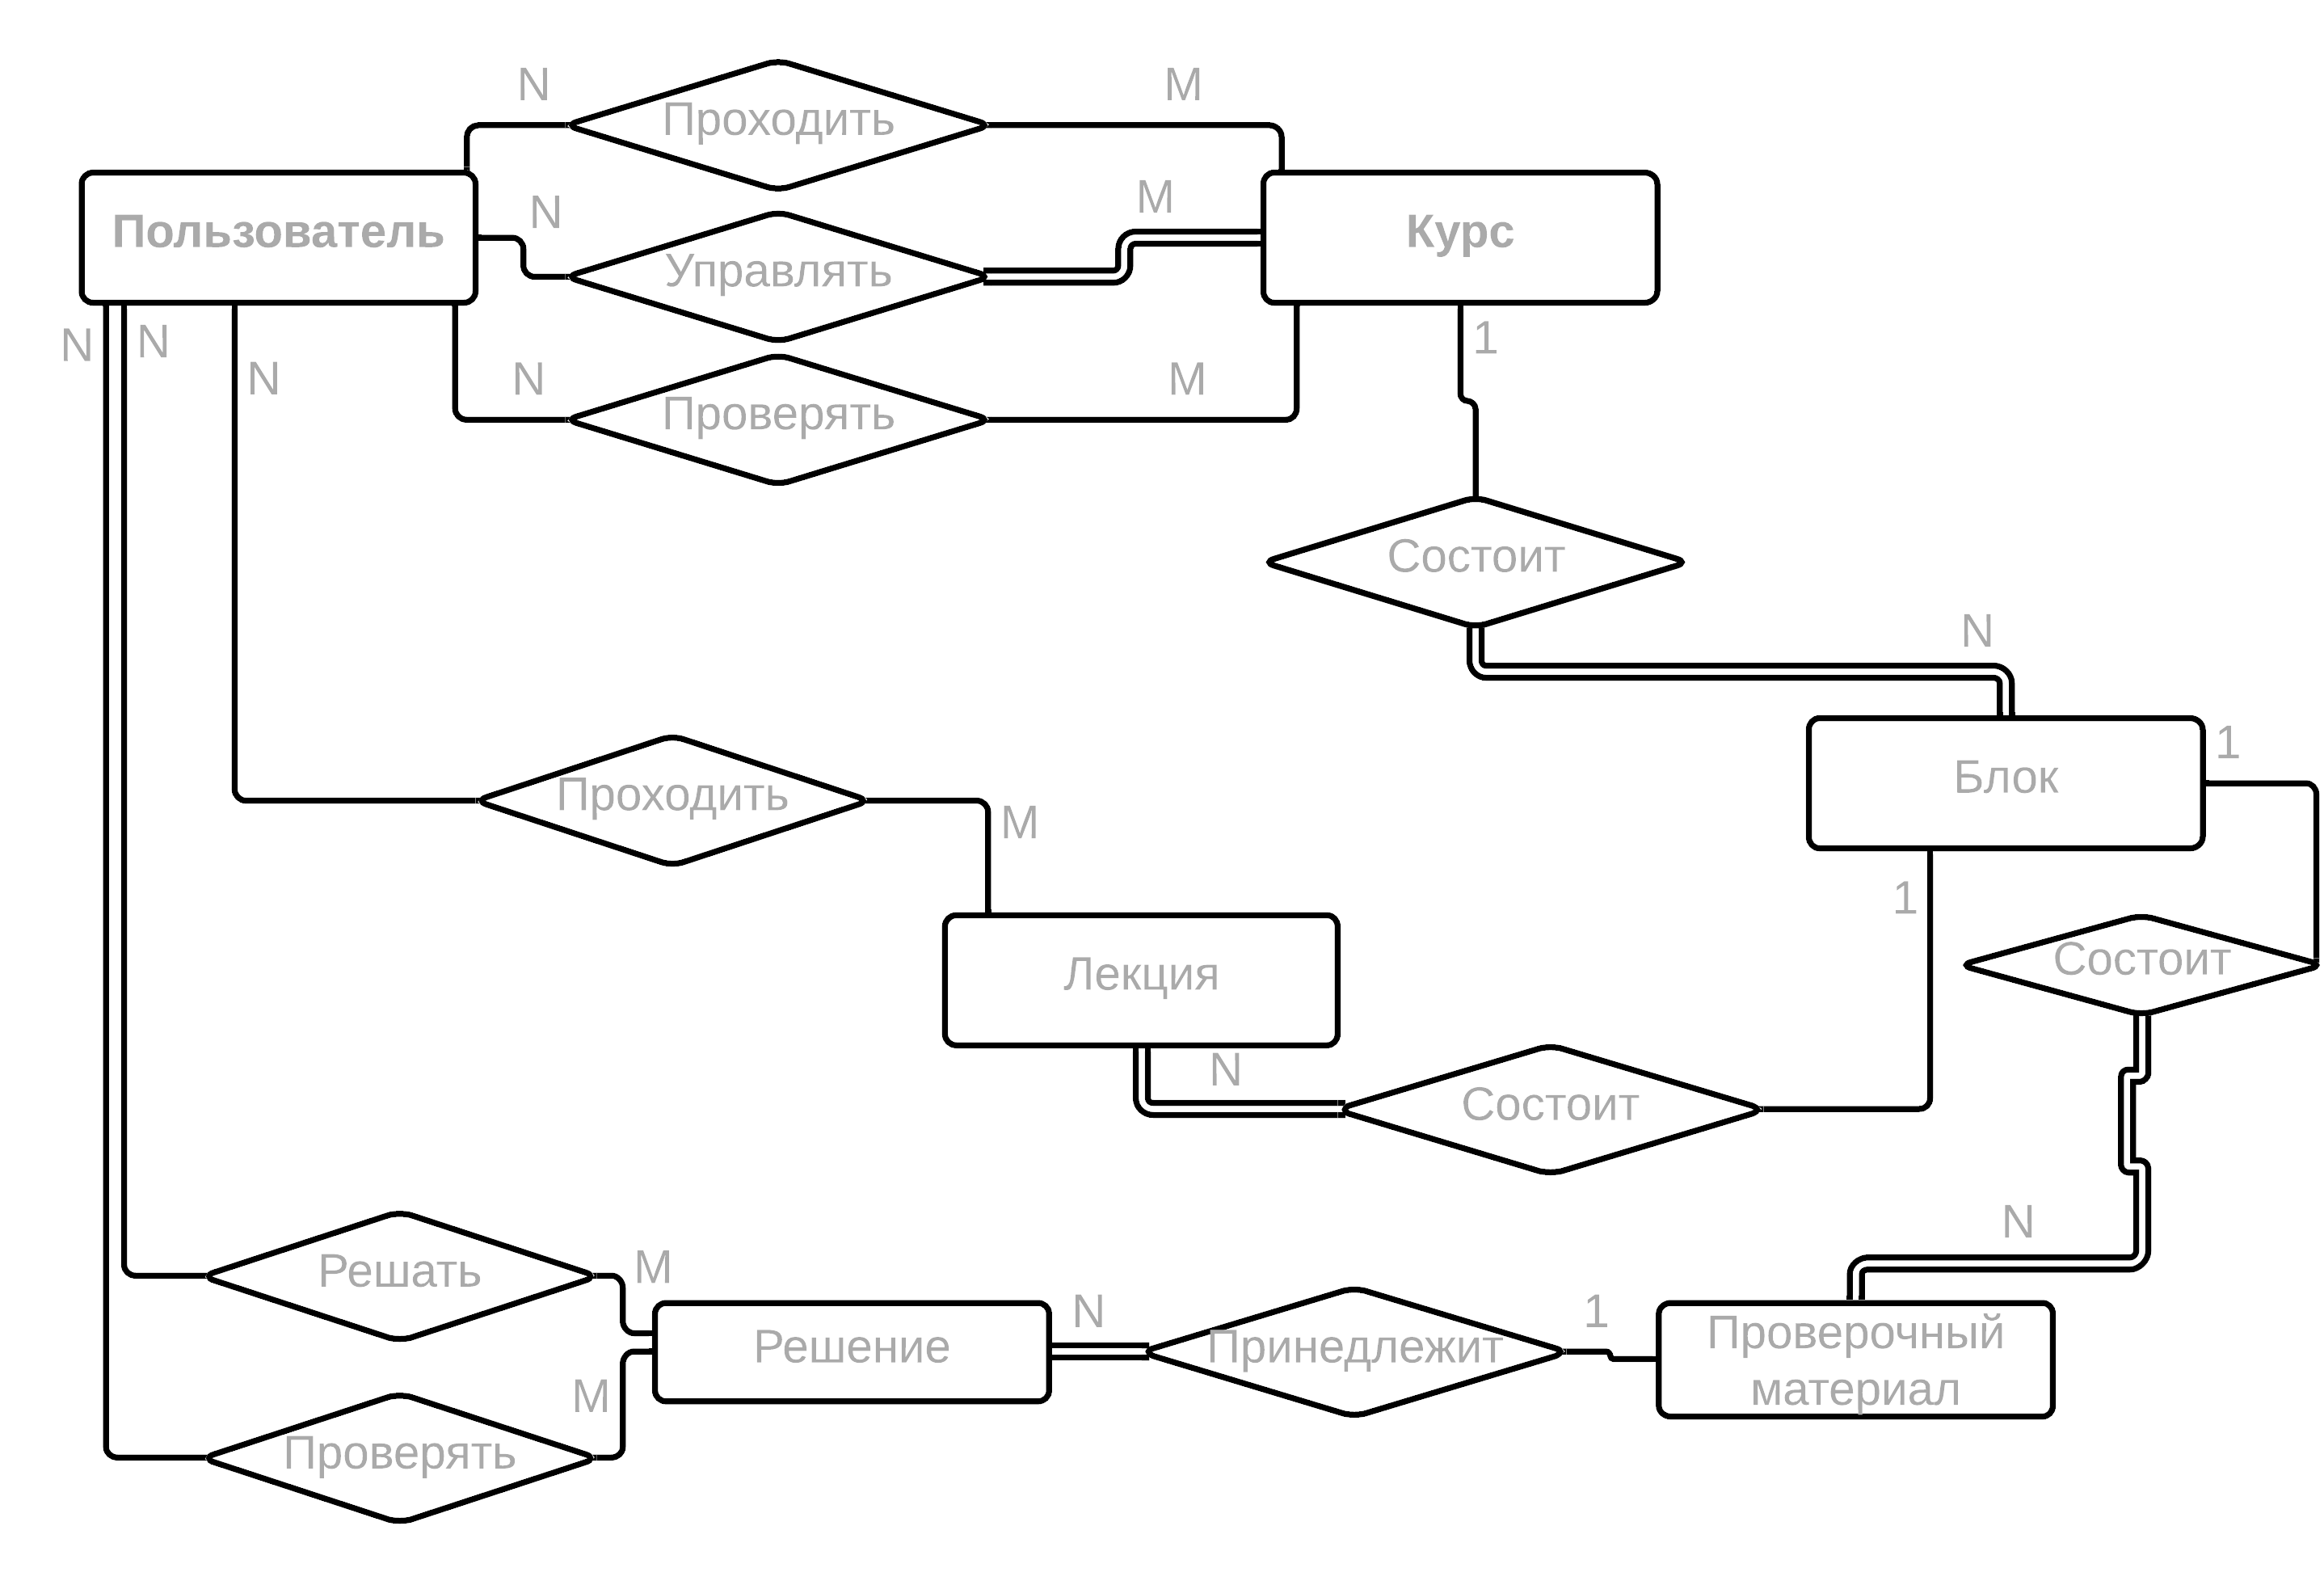
\includegraphics[width=\linewidth]{schemas/ER}
	\caption{ER диаграмма}\label{img:db_ER}
\end{figure}

\section{Анализ информационных задач и круга пользователей системы}

Определим группы пользователей, их основные задачи и запросы к БД:

\begin{enumerate}
	\item Администратор ресурса
	\begin{itemize}
		\item Регистрация новых пользователей;
		\item Создание новых курсов;
		\item Привязка преподавателей к курсу;
		\item Управление платформой и курсами.
	\end{itemize}

	\item Преподаватель курса
	\begin{itemize}
		\item Регистрация и приглашение новых учеников и ассистентов на курс;
		\item Создание и редактирование информации о курсе (блоки, лекции, проверочные работы);
		\item Просмотр прогресса учеников по курсу;
		\item Проверка работ учащихся курса.
	\end{itemize}

	\item Ассистент курса
	\begin{itemize}
		\item Проверка работ учеников на подконтрольных курсов;
		\item Просмотр результатов собственной проверки.
	\end{itemize}

	\item Ученик
	\begin{itemize}
		\item Запись на существующие курсы;
		\item Чтение и фиксация прогресса по лекциям;
		\item Доступ к материалам проверочных работ;
		\item Многократное выполнение и отправка попыток на проверку;
		\item Доступ к результатам проверки.
	\end{itemize}
\end{enumerate}

\section{Определение требований к операционной обстановке}
На основе результатов анализа предметной области можно приблизительно оценить объём памяти, требуемой для хранения данных.
Примем ориентировочно, что:
\begin{itemize}
	\item В системе зарегистрировано 1000 пользователей (по 0.25К на запись);
	\item В системе создано 10 курсов, каждый из которых состоит в среднем из 32 блоков (0.2К на информацию о курсе);
	\item Каждый блок состоит из 5 лекционных материалов и 2 проверочных работ (0.1К на информацию о блоке);
	\item Каждая лекция содержит 5К текстовой информации;
	\item Каждый проверочный материал занимает 1К;
	\item Ученик записан в среднем на 2 курса;
	\item Ученик читает все лекции и решает в среднем 2 раза каждое задание (0.1К на чтение лекции и 3К на попытку решения).
\end{itemize}

Тогда объем памяти, занимаемый базой данных будет примерно равен:
\begin{multline*}
2 \times( 10 \times ((32 \times (5 \times 5K + 2 \times 1K) + 0.1K) + 0.2K) + \\ 
+ 1000 \times (2 \times 32 \times (5 \times 0.1K + 2 \times 2 \times 3K) + 0.25K)) = 1617786K	\approx 1.5G
\end{multline*}

\section{Выбор СУБД и других программных средств}
Будем писать на PostgreSQL.

\section{Преобразование ER–диаграммы в схему базы данных}

\begin{figure}[H]
	\centering		
	\includegraphics[width=\linewidth]{schemas/RDB}
	\caption{Схема базы данных}\label{img:RDB}
\end{figure}

\subsection{Составление реляционных отношений}

%1. Пользователь. Атрибуты: ФИО, логин, пароль, пол, почта;

Потенциальными ключами отношения ПОЛЬЗОВАТЕЛЬ являются поля логин и адрес электронной почты. Все они занимают достаточно много места. Введём суррогатный первичный ключ Номер пользователя.

\begin{table}[H]
	\begin{flushleft} 
		\tablecaption{\label{tab:UserV1} Схема отношения ПОЛЬЗОВАТЕЛЬ (User) }
	\end{flushleft}
\begin{adjustbox}{width=\linewidth}
\begin{tabular}{|l|l|c|l|}
	\hline
	Содержание поля        & Имя поля & Тип, длина & Примечания                          \\ \hline
	Номер пользователя     & U\_ID     &    N(4)    & \textbf{суррогатный первичный ключ} \\ \hline
	Фамилия, имя, отчество & U\_FIO    &   V(100)   & обязательное поле                   \\ \hline
	Дата рождения          & U\_BORN   &    Date    & обязательное поле                   \\ \hline
	Пол                    & U\_GENDER &    C(1)    & обязательное поле, 'м' или 'ж'      \\ \hline
	Логин                  & U\_LOGIN  &   V(30)    & обязательное поле                   \\ \hline
	Почта                  & U\_MAIL   &   V(30)    & обязательное поле                   \\ \hline
	Пароль                 & U\_PASS   &   V(30)    & обязательное поле                   \\ \hline
\end{tabular}
\end{adjustbox}
\end{table}

%2. Курс. Атрибуты: названия, категория, видимость;

Потенциальным ключом отношения КУРС является поле название. Оно занимает достаточно много места. Введём суррогатный первичный ключ номер курса.

\begin{table}[H]
	\begin{flushleft} 
		\tablecaption{\label{tab:CourseV1} Схема отношения КУРС (Course) }
	\end{flushleft}
	\begin{tabular}{|l|l|c|l|}
		\hline
		Содержание поля & Имя поля     & Тип, длина & Примечания                          \\ \hline
		Номер курса     & C\_ID         &    N(4)    & \textbf{суррогатный первичный ключ} \\ \hline
		Название        & C\_NAME       &   V(100)   & обязательное поле                   \\ \hline
		Категории       & C\_CATEGORY   &   V(100)   & обязательное поле                   \\ \hline
		Видимость       & C\_VISIBILITY &    BOOL    & обязательное поле, default FALSE    \\ \hline
	\end{tabular}
\end{table}

%3. Блок. Атрибуты: тема, видимость;

У отношения БЛОК нет потенциального ключа, поэтому введём суррогатный первичный ключ номер блока.

\begin{table}[H]
	\begin{flushleft} 
		\tablecaption{\label{tab:BlockV1} Схема отношения КУРС (Block) }
	\end{flushleft}
	\begin{tabular}{|l|l|c|l|}
		\hline
		Содержание поля & Имя поля & Тип, длина & Примечания                          \\ \hline
		Номер блока     &  B\_ID        &    N(4)    & \textbf{суррогатный первичный ключ} \\ \hline
		Тема            &  B\_THEME        &   V(100)   & обязательное поле                   \\ \hline
		Видимость       &  B\_VISIBILITY        &    BOOL    & обязательное поле, default FALSE    \\ \hline
		Курс            &  B\_COURSE        &    N(4)    & внешний ключ (к Course)             \\ \hline
	\end{tabular}
\end{table}

%4. Лекция. Атрибуты: название, содержание, продолжительность, видимость;

У отношения ЛЕКЦИЯ нет потенциального ключа, поэтому введём суррогатный первичный ключ номер лекции.

\begin{table}[H]
	\begin{flushleft} 
		\tablecaption{\label{tab:LectureV1} Схема отношения ЛЕКЦИЯ (Lecture) }
	\end{flushleft}
\begin{adjustbox}{width=\linewidth}
	\begin{tabular}{|l|l|c|l|}
		\hline
		Содержание поля   & Имя поля     & Тип, длина & Примечания                          \\ \hline
		Номер лекции      & L\_ID         &    N(4)    & \textbf{суррогатный первичный ключ} \\ \hline
		Название          & L\_NAME       &   V(100)   & обязательное поле                   \\ \hline
		Содержание        & L\_CONTENT    &    TEXT    &                                     \\ \hline
		Продолжительность & L\_DURATION   &  INTERVAL  &                                     \\ \hline
		Видимость         & L\_VISIBILITY &    BOOL    & обязательное поле, default FALSE    \\ \hline
		Блок              & L\_BLOCK      &    N(4)    & внешний ключ (к Block)              \\ \hline
	\end{tabular}
\end{adjustbox}
\end{table}
%5. Проверочный материал. Атрибуты: название, максимальный балл, продолжительность, видимость;

У отношения ПРОВЕРОЧНЫЙ МАТЕРИАЛ нет потенциального ключа, поэтому введём суррогатный первичный ключ номер проверочного материала.

\begin{table}[H]
	\begin{flushleft} 
		\tablecaption{\label{tab:TestMaterialV1} Схема отношения ПРОВЕРОЧНЫЙ МАТЕРИАЛ (TestMaterial) }
	\end{flushleft}
\begin{adjustbox}{width=\linewidth}
	\begin{tabular}{|l|l|c|l|}
		\hline
		Содержание поля              & Имя поля     & Тип, длина & Примечания                          \\ \hline
		Номер проверочного материала & T\_ID         &    N(4)    & \textbf{суррогатный первичный ключ} \\ \hline
		Название                     & N\_NAME       &   V(100)   & обязательное поле                   \\ \hline
		Задание                      & N\_TASK       &    TEXT    & обязательное поле                   \\ \hline
		Максимальный балл            & N\_MAX        &    N(4)    & обязательное поле                   \\ \hline
		Продолжительность            & N\_DURATION   &  INTERVAL  &                                     \\ \hline
		Видимость                    & N\_VISIBILITY &    BOOL    & обязательное поле, default FALSE    \\ \hline
		Блок                         & N\_BLOCK      &    N(4)    & внешний ключ (к Block)              \\ \hline
	\end{tabular}
\end{adjustbox}
\end{table}

%6. Решение. Атрибуты: содержание, оценка.

У отношения ПОПЫТКА нет потенциального ключа, поэтому введём суррогатный первичный ключ номер решения.

\begin{table}[H]
	\begin{flushleft} 
		\tablecaption{\label{tab:AttemptV1} Схема отношения ПОПЫТКА (Attempt) }
	\end{flushleft}
	\begin{tabular}{|l|l|c|l|}
		\hline
		Содержание поля & Имя поля  & Тип, длина & Примечания                          \\ \hline
		Номер решения   & A\_ID      &    N(4)    & \textbf{суррогатный первичный ключ} \\ \hline
		Содержание      & A\_CONTENT &    TEXT    & обязательное поле                   \\ \hline
		Оценка          & A\_MARK    &    N(4)    &                                     \\ \hline
		Дата сдачи      & A\_DATE    &    Date    & обязательное поле, default NOW()    \\ \hline
		Автор попытки   & A\_AUTHOR  &            & внешний ключ (к User)               \\ \hline
		Проверяющий     & A\_CHECKER &            & внешний ключ (к User)               \\ \hline
		Задание         & A\_TASK    &            & внешний ключ (к TestMaterial)       \\ \hline
	\end{tabular}
\end{table}

%7. Участие. Атрибуты: роль, номер пользователь, номер курса.

У отношения УЧАСТИЕ нет потенциального ключа, поэтому введём суррогатный первичный ключ номер решения.

\begin{table}[H]
	\begin{flushleft} 
		\tablecaption{\label{tab:ParticipationV1} Схема отношения УЧАСТИЕ (Participation) }
	\end{flushleft}
	\begin{tabular}{|l|l|c|l|l|}
		\hline
		Содержание поля & Имя поля & Тип, длина & \multicolumn{2}{l|}{Примечания} \\ \hline
		Роль & P\_ROLE & С(10) & \multicolumn{2}{l|}{обязательное поле} \\ \hline
		Номер пользователя & P\_USER & N(4) & \begin{tabular}[c]{@{}l@{}}
			  внешний ключ   \\
			(к User)
		\end{tabular} & \multirow{2}{*}{\begin{tabular}[c]{@{}l@{}}\textbf{составной}\\ \textbf{первичный} \\ \textbf{ключ}\end{tabular}} \\ \cline{1-4}
		Номер курса & P\_COURCE & N(4) & \begin{tabular}[c]{@{}l@{}}внешний ключ \\ (к Course)\end{tabular} &  \\ \hline
	\end{tabular}
\end{table}

%8. Участие. Атрибуты: роль, номер пользователь, номер курса.

У отношения ПРОЧИТАННЫЕ ЛЕКЦИИ нет потенциального ключа, поэтому введём суррогатный первичный ключ номер решения.

\begin{table}[H]
	
	\begin{flushleft} 
		\tablecaption{\label{tab:LectionRead} Схема отношения ПРОЧИТАННЫЕ ЛЕКЦИИ (LectionRead) }
	\end{flushleft}
	\begin{adjustbox}{width=\linewidth}
	\begin{tabular}{|l|l|c|l|l|}
		\hline
		Содержание поля & Имя поля & Тип, длина & \multicolumn{2}{l|}{Примечания} \\ \hline
		Номер пользователя & LR\_USER & N(4) & \begin{tabular}[c]{@{}l@{}}внешний ключ \\ (к User)\end{tabular} & \multirow{2}{*}{\begin{tabular}[c]{@{}l@{}}\textbf{составной}\\ \textbf{первичный} \\ \textbf{ключ}\end{tabular}} \\ \cline{1-4}
		Номер лекции & LR\_NUMLECTURE & N(4) & \begin{tabular}[c]{@{}l@{}}
			  внешний ключ    \\
			(к номер Lecture)
		\end{tabular} &  \\ \hline
	\end{tabular}
\end{adjustbox}
\end{table}

%\newpage 
%\renewcommand{\refname}{{\normalsize СПИСОК ИСПОЛЬЗОВАННЫХ ИСТОЧНИКОВ}} 
%\centering 
%\begin{thebibliography}{9} 
%	\addcontentsline{toc}{section}{\refname} 
%	\bibitem{sql} Beaulieu A. Learning SQL: Master SQL Fundamentals. – " O'Reilly Media, Inc.", 2009.
%	
%\end{thebibliography}

\end{document} % конец документа